
\documentclass[11pt]{article}

\usepackage{url}
\usepackage{hyperref}
\usepackage{graphicx}
\usepackage{grffile}
\usepackage{xcolor}

\graphicspath{{figs/}}
\begin{document}

\title{Mathematics with the HP48G Calc}
\author{GNU Author}
\date{2006 February}
\maketitle

\section{Linear Systems}
System of linear equations is a set of equations. The equations have the same set of variables.

\subsection{Example 1}
A first basic example is given as follows:
\begin{itemize}
\item Linear system (1)
\begin{itemize}
\item $ 3x + 2y   -z = 1 $
\item $ 2x - 2y  +4z = -1 $
\item $ -x + 0.5y -z = 0 $
\end{itemize}
\end{itemize}


\begin{itemize}
\item The solution is:
\begin{itemize}
\item $ x = 1 $
\item $ y = -2 $
\item $ z = -2 $
\end{itemize}
\end{itemize}



\begin{itemize}
\item The solution with HP48g with image of the calculator:
\begin{itemize}
\item Several screenshots of the calculator are given. First it illustrates entering the two matrix, which will allow to solve the system.
\item Press "Solve" allows the HP48G to calculate and return the solution in form of a matrix.
\end{itemize}
\end{itemize}


\bigskip
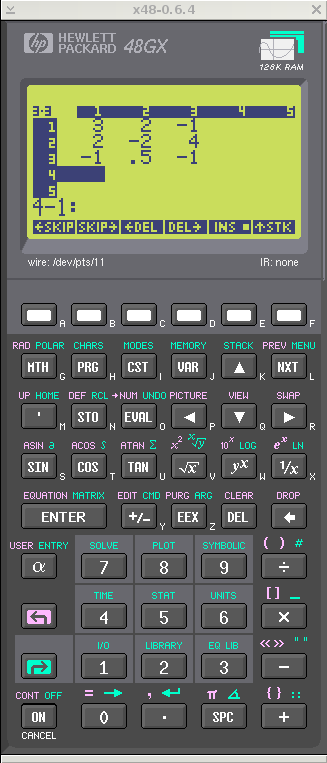
\includegraphics[scale,height=0.33\textheight]{20180422143232-linear01-p1.png}
~
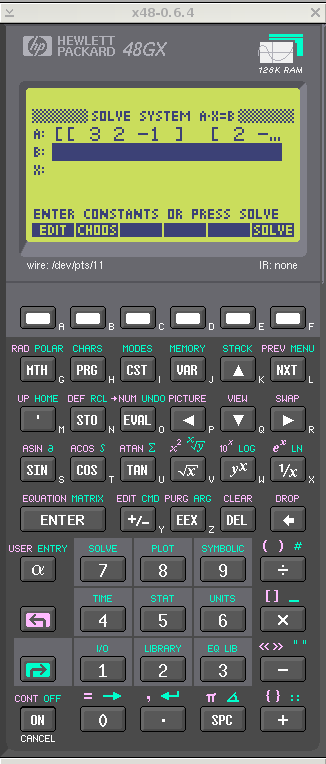
\includegraphics[scale,height=0.33\textheight]{20180422143232-linear01-p2.png}
~
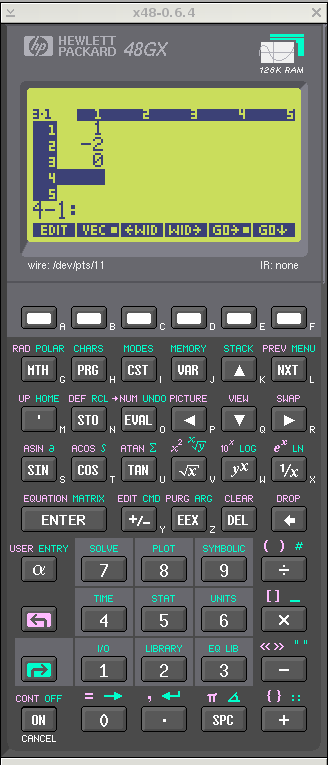
\includegraphics[scale,height=0.33\textheight]{20180422143232-linear01-p3.png}
\bigskip

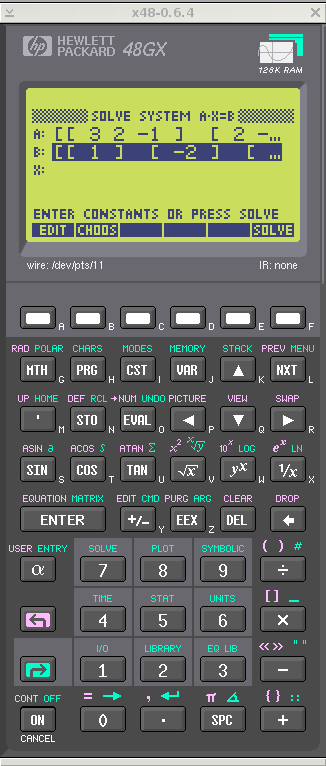
\includegraphics[scale,height=0.33\textheight]{20180422143232-linear01-p4.png}
~
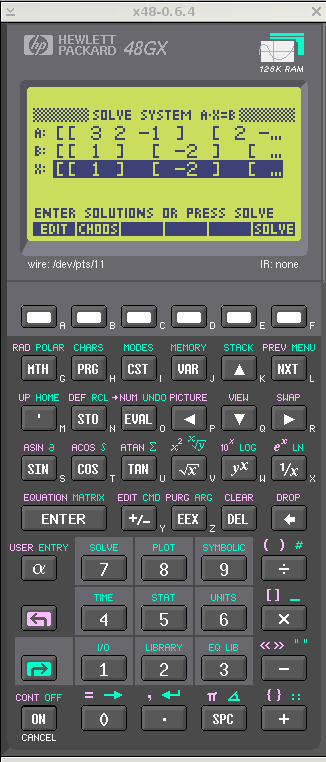
\includegraphics[scale,height=0.33\textheight]{20180422143232-linear01-p5.png}
~
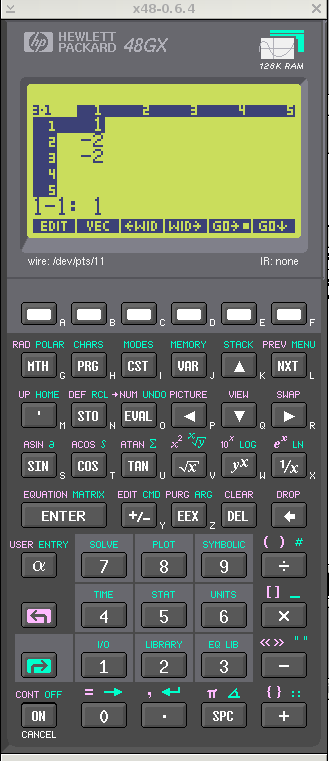
\includegraphics[scale,height=0.33\textheight]{20180422143232-linear01-p6.png}

\end{document}
